\documentclass[pageno]{jpaper}

%replace XXX with the submission number you are given from the ASPLOS submission site.
\newcommand{\asplossubmissionnumber}{XXX}

\newcommand{\Op}{\mathrm{\mathbf{Op}}}
\newcommand{\Ev}{\mathbf{E}}

\usepackage[normalem]{ulem}

\usepackage{verbatim}   % Needed for the "comment" environment to make LaTeX
                        % comments
\usepackage{vector}     % Allows "\bvec{}" and "\buvec{}" for "blackboard"
                        % style bold vectors
\usepackage{listings}
\usepackage{lstpatch}
\lstset{captionpos=b,
        frame=tb,
        basicstyle=\scriptsize\ttfamily,
        showstringspaces=false,
        keepspaces=true}

\hypersetup{urlcolor=blue, colorlinks=true}

\usepackage{tikz}  % for drawing graphs and diagrams
\usetikzlibrary{
  shapes.multipart,
  shapes.geometric,
  arrows,
  fit,
  matrix,
  positioning,
  shapes.callouts,
  shapes.arrows,
  calc
}

\usepackage{pgfplots}
\pgfplotsset{compat=1.10}
\usetikzlibrary{shapes.geometric,arrows,fit,matrix,positioning}

\definecolor{myyellow}{RGB}{245,177,0}
\definecolor{mysalmon}{RGB}{255,145,73}

\usepackage{amsmath}
\usepackage{amssymb}
\usepackage{mathtools}
\DeclarePairedDelimiter\ceil{\lceil}{\rceil}
\DeclarePairedDelimiter\floor{\lfloor}{\rfloor}

\begin{document}

\title{
Using Persistent Data Models to Automate Parallelism under Synchronization Requirements}

\date{Aug 15, 2016}
\maketitle

\thispagestyle{empty}

\begin{abstract}
We implement a vector, using a bit-partitioned trie, that allows for consistent
concurrent reading and writing between multiple tasks under some constraints on
the properties of those tasks. This data structure, along with a work queue and
a framework for resolving operations that conflict with each other, yields a
method for automatically parallelizing a graph of tasks that may have
synchronization requirements under traditional memory models. We test the
method against a variety of shared-memory parallelism techniques including C++
threads, AVX registers, and OpenMP directives by invoking repeated reduce and
foreach operations on an initial random input in the MB to GB scale. Our method
achieves comparable weak and strong scaling results and similar raw
performance. It beats serial implementations on a dual-core machine and runs
only 4\% to 50\% slower than the best-performing technique on up to 8 cores,
without requiring manual synchronization between steps and while providing
greater algorithmic flexibility.
\end{abstract}

\section{Introduction}
Sometimes, data and their corresponding algorithms have a ``trivially
parallelizable'' characteristic (e.g. domain decomposition of the region of
interest in a simulation), where processors have, and write to, disjoint sets of
data. But, other tasks may require requiring either data sharing across sets or
a reconfiguration of those sets. For example, matrix multiplications require a
row/column ordering of processors, but this does not minimize interprocessor
boundaries as in an ideal domain decomposition. Furthermore, matching these sets
to other overlaid structures for computation, such as meshes, presents further
difficulties. Even providing a balanced decomposition of data onto processors
can itself prove elusive and challenging, and exchange of data across the
resulting boundaries may require intricate and complex handling. In this way,
data races have emerged as a problem for both shared and distributed memory
parallelism in settings where multiple cores write and read the same data,
necessitating synchronization. 

More current technologies for memory management in the
context of concurrency and parallelism have not integrated into the most popular
software, for historical but practical reasons: issues of compatibility,
maintainability, scalability, reliability, complexity, efficiency, and more have
prevented an elegant transition \cite{kokkos_port}. In specialized settings,
implementations of such algorithms have emerged \cite{erlang_hpc}
\cite{clojure_hpc}. But, this work often lacks comparisons to traditional
programs in terms of performance metrics and remains specialized and
disconnected from practice and end users. Furthermore, these implementations
often do not take advantage of the touted feature-sets of their languages or
environments, such as algorithmic immutability (realized as persistency in
Clojure), lazy evaluation, a functional programming perspective of state, and
abstraction. Books, manuals, and tutorials will recommend using an exposed
low-level interface to achieve higher performance, defeating the purpose of
using a higher-level language or environment. Haskell suggests writing code in
its internal representation to avoid situations where its compiler cannot
appropriately optimize code \cite{haskell_opt}.

When new theoretical improvements emerge in high performance computing
algorithms, programmers should not feel limited by the tools they have in
implementing, testing, benchmarking, and analyzing those algorithms in
real-world situations. Scientists should have tools that let them express their
ideas clearly and readily while also taking advantage of modern hardware and
software. I will describe and sketch the implementation
of a parallel container (that can be realized as a vector, hash map, b-tree, or
any other such data structure) in C++ with the following characteristics:
\begin{enumerate}
    \item Automoatic synchronization of reads and writes in shared memory
        without data races, and a model for how the same can be done in a
        distributed memory system;
    \item Usable as a drop-in replacement for a C++ standard library vector for
        a restricted set of member functions and inner types and operations on
        those types;
    \item Asymptotically identical runtimes for the operations when used in
        serial and the corresponding expected improvements when used in
        parallel;
    \item An interface for arbitrarily partitioning the vector across
        processors;
    \item An interface for extending the set of inner types that can be used;
    \item A model for generalizing the set of inner types and operations on
        those types used.
\end{enumerate}

I will also provide the implementation of the following actual parallel
algorithms using an implementation of this container to provide examples
of how it will work, and I will show how they correspond to current
implementations that use manual concurrency control and parallelism techniques:
\begin{enumerate}
    \item A ``foreach'' operation that takes the vector and applies one
        operation to all items in the vector (either a unary operation or a
        binary operation with another supplied input), resulting in an output
        vector of the same size;
    \item A ``reduce'' operation that takes the vector and applies one operation
        to all items in the vector, resulting in a final output value;
\end{enumerate}

\section{Background}

\subsection{Motivating Automated Parallelism Given the State of Modern
Computational Tools}
Moore's law dictates that the number of computational components per unit space
(such as an integrated circuit) doubles per unit time.  These
components cannot necessarily be used to accelerate the rate of sequential
computation, and instead, the decrease in component size has been utilized by
developing multicore hardware. Further spatial limitations prevent shared memory
arrangements for large numbers of processors greater than around about 64 for
standard CPUs and about 1000 for new ``manycore'' processors \cite{manycore}.

Distributed memory hardware configurations, referred to as clusters, involve the
arrangement of many computers, referred to as nodes, that have their memory
interconnected by some communication protocol. They may contain over 1 million
nodes \cite{top500}. Due to the plethora of nodes, computation time within
individual nodes decreases relative to the communication time required to send
data between nodes. Because of this new bottleneck, developing
communication-mitigating algorithms has become a popular area of interest. Some
work involves modifying parallel algorithms such that the resulting algorithm
requires less communication \cite{strassen_comm_opt}. Other work involves
``pipelining'' algorithms such that communication and computation can overlap in
time -- the program dedicates some threads within a node to performing
communication, while other threads carry out any computation that does not rely
on unreceived data \cite{gmres_pipe}.  More generally, methods that reduce the
need for synchronization between nodes can improve parallel CPU utilization.

Using
algebraic and combinatorial code analysis, optimization, and generation
techniques, methods like polyhedral optimization and Decoupled Software
Pipelining (DSWP) have achieved automation of pipelining (and more generally the
parallelization of loops with data dependencies between iterations)
\cite{polyopt} \cite{dswp}. The development and use of these methods stems from
an implicit yet nonessential sequential ordering in the implementation of the
serial version of the algorithms upon which these methods operate. These
nonessential orderings derive from the procedural nature characteristics of the
languages used to implement the algorithms in question.

\subsubsection{Related Existing Control Techniques}
In transactional memory blocks of code are
marked as ``atomic'', and code executes in parallel with no explicit concurrency
control. If code within an atomic block interleaves with other code in a harmful
way, then the block (called a ``transaction'' in this context) restarts from the
beginning, discarding all modifications made since. Clojure has an advanced STM
system that allows the user to specify certain equivalences, allowing the STM
system to complete even if the prescribed ordering does not match the execution
ordering exactly. A user can specify that a function application commutes in time
with itself -- for example, a user can specify that an increment operation on a
counter commutes, so that any number of increments, in any order, performed in
transactions on that particular value will not cause transactions to restart. Further
flexibility comes in the form of an \texttt{ensure} operation that Clojure uses to
require that a read value has not been mutated by that point. Clojure uses the
\texttt{alter} and \texttt{ref-set} operations as its primary read-write and write
operations within transactions. Finally, Clojure uses ``agents'' to perform
asynchronous operations on values without guaranteeing when other threads will
see those writes. Agents have their own set of functions that provide
flexibility: \texttt{await} blocks waiting for an agent, \texttt{set-validator}
associates some kind of check with the mutation of agents, \texttt{add-watch}
registers observers to trigger when an agent mutates, and \texttt{deref} and
\texttt{send} allow for read and read/write operations to interact properly with
those possibilities.

Clojure has a smorgasbord of other concurrency control mechanisms, ranging from
``reducers'' (which both amount to generalized, parallel SIMD operations) to
``transducers'' to ``futures'' and more.

\subsection{Leveraging Immutability for Parallelism}

Clojure serves as a good example for how immutability can assist in automated
parallelism. It provides persistent data structures that appear immutable from
any reference, but can also accrue updates from those references, updates that
eventually propagate to those references. It does this without making entire
copies of those data structures, and instead by using pointers to catalog to
portions of the data structure that have not changed from any reference. An
excellent informal description of how persistent vectors work can be found at
Niklas D'orange's website \cite{persvec1}, and a detailed description of an
optimized persistent vector can be found in the ICPF 2015 conference proceedings
\cite{rrb_vec}.  Clojure’s persistent vector uses a b-trie for its internal
representation. The values in the vector are stored in leaves. If some reference
modifies the vector, it identifies the leaf of the trie that should contain the
modify value, creates a new version of that leaf with the updated value, and
creates a new root (and hence, a new trie) with the structure that results in
the modified vector without having to duplicate anything except the other parts
of the modified leaf. Sometimes new leaves (and the corresponding internal nodes
and branches to that leaf) must be created as well, and sometimes empty leaves
and internal nodes and branches must be pruned. Clojure uses 32 children per
node, and achieves $O(\log_{32} n$) (what they consider effectively $O(1)$)
time for \texttt{append}, \texttt{update}, \texttt{lookup}, and \texttt{subvec},
as a mutable vector does. Even with this generous reading ($\log_{32} n \leq c$
for some constant upper-bound $c$), the persistent version does incur a constant
overhead involved with creating this representation of the vector and with
performing the maintenance of this trie. Clojure uses numerous tricks to
optimize this data structure. First, it uses bit partitioning, where the trie
branches based on 5 possible bit values (generating 32 branches per node). By
doing this, Clojure provides a means for looking up elements in a vector tied to
its internal representation. Looking at 5 bits at a time, the algorithm for
lookup walks through the internal nodes of the trie until it reaches a leaf,
where the value is stored. It furthermore uses a tail node, pointed to directly
by the root, to optimize modifications near the end of the vector.

\subsubsection{Transient Vectors: Relaxing Immutability When Helpful}
Transient versions of persistent vectors modify values directly. Persistent
vectors can be copy-constructed to transient vectors, and transient vectors that
have been modified are invalidated such that using them after modification
results in undefined behavior. Nodes and leaves are given IDs that correspond
to the reference that created them, and the transient vector can safely mutate
these. Finally, transient vectors can be copy-constructed back to persistent
vectors, where that reference behaves as any other persistent vector would,
invalidating the transient from which it was copied. By doing this, a stream of
unobserved mutations can take place without sacrificing the guise of
immutability. D'orange's masters thesis discusses optimizations of Relaxed Radix
Balanced Trees (RRB-Trees) through transience \cite{lorange2014rrb}.

\subsubsection{Persistency to Automate Concurrency Control without Race Conditions}
In a parallel application, processors can read and write to shared data. Before
performing a read of some data, a processor may want an updated version of that
data, or a version that corresponds to a certain point in a global ordering of
events, even if it stores that data in a persistent data structure. It may
hypothesize or expect that the data has changed and specifically want an updated
value. When this happens, it has to verify that the other process  has completed
its operations. Consider that each process converts an initial persistent vector
into a transient vector, where each process's vector gets its own ID. Then, that
process's transient vector sees its own modifications transiently, in real time,
but sees a persistent, immutable copy of the values other processes may have
modified. With the knowledge of both the values a process does not own and the
values it needs to read, any given process can safely obtain the most updated
version of a value: by reading the values it owns as it wishes, and by waiting
for other processes only when necessary. If multiple processes write to the same
locations in the vector, the situation becomes more complicated, and the values
must somehow be reconciled.

\section{Theoretical Groundwork for Automated Parallel Methods}

\subsection{Motivation: Parallelism Necessitates Concurrency Control}
Consider that in the general case of a program intended for parallel execution,
the potential arises for two processors to perform computations that conflict
with each other. Specifically, when two processors access the same memory
location and at least one of them performs a write at that location, a conflict
arises, because the both code does not prescribe a global ordering of those
accesses and the order changes the outcome. Hence, this conflict results in a
program state that could potentially produce an incorrect result. Conflicts
occur when parallel programs cannot be mapped to unique sequential programs due
to their asynchronous properties -- at least one of the orders in which the
instructions could be executed, in combination with the program state, yielded
an invalid program state at a later point in time.

In the most general case, it may prove challenging or impossible to prevent or
resolve these conflicts without relying on synchronization mechanisms that
prevent full utilization of parallel execution. But, if certain constraints are
applied to
\begin{enumerate}
    \item the operations that the processors will execute, and
    \item the read/write access patterns upon the data with which those
        operations will interact,
\end{enumerate}

the task becomes feasible. This in hand with a clever organization of memory
will yield automated parallelism methods.

\subsection{Groundwork for Minimal Concurency Control Mechanisms}
The following will assist in the description of concurrency control schemes that
come afterward.

\subsubsection{Terms, Definitions, and Assumptions}
We shall specify constraints for operations that processors may execute in
parallel in such a way that conflicts can be detected and eventually resolved.
These constraints give way to relaxations of the execution ordering of those
operations.

Each relaxation specifies a set of operations $\Op_{i}$ that contains all
functions that it allows. We assume that the operations have the form $\Op:
\mathbb{R}^{n} \mapsto \mathbb{R}$. If an operation effectively produces many
values, we model it as a series of operations that take the same inputs.  The
constraints will apply to the set $\Op$. The constraints may involve restricting
the domain to a subset of the general case above. In a practical setting, the
function's range will be the values allowed by a given numeric data type, such
as \texttt{uintXX}, \texttt{intXX}, or \texttt{float{XX}}, where $\texttt{XX}
\in {8, 16, 32, 64}$. We will refer to the inputs and output of a function as
\emph{values}, and in code, we will give them the general type \texttt{val}.

Then, we will provide a function $C_i$ which will identify a conflict, and a
function $R_i$ that will provide a way to resolve conflicts that arise.

Finally, we will define the set $St_{i,t}$ as the relevant subset of the program
state after $t$ operations. Here, relevant means that this program state works
in isolation with regard to all other operations taking place within the
program: no outside operations are reading or writing values in $St$;
furthermore, operations happening within $St$ do not read or write values
outside of $St$ either. Sometimes the program state is undefined for a certain
$t$, but we will place limitations on when this is acceptable \cite{timeclocks}.
Unless an operation produces no output, it modifies the program state via its
output.

Consider that any variable in a program has a set of dependencies. A dependency
is another variable used to compute the first's value at some point during the
computation. Adjacent dependencies appear immediately in these computations, and
those may have their own dependencies as well. Construct a dependency graph $G$
for a variable in a subroutine. The graph begins as a single node, just the
variable itself; call it $v_0$. Iterate through the execution paths of the
program until the variable receives an assignment of some value. If the value is
constant and does not come from the evaluation of an expression, do not modify
the graph. If the value comes from the result of an expression, take each
variable inside the expression and add them to the graph, drawing a directed
edge from each of them to $v_0$. Continue doing this until $v_0$ shares an edge
with every variable contained in an expression assigned to $v_0$. Then, repeat
the process for each of these newfound dependencies. If the assignment to $v_0$
results from a function call, then this process must be repeated with the return
value of the function in question, which itself serves as the sole direct
dependency of $v_0$ from the call. Note that the graph may have cycles. In fact,
very simple subroutines have cycles. For example, incrementing a counter has one
node and an edge connected to itself -- a loop. Now, take any paths for which
each node in the path has only a single incoming and outgoing edge and compress
them into a single node. These paths result from inherently serial computations.
The number of intermediate variables used to represent these computations is
incidental and nonessential to the graph's meaning. Such subgraphs cannot be
parallelized, as each operation depends exactly on the preceding one. 

Consider a partition of the edges of the compressed graph by its connected
subgraphs. These subgraphs can be executed independently, yielding parallelism.
Now consider removing an arbitrary node $n$ from the graph. If the number of
subgraphs increases due to the removal of $n$, then the newly-generated
subgraphs correspond to sections of the subroutine that are computationally
independent. Without loss of generality, say there are 2 such newly-generated
subgraphs $P$ and $Q$. There are three cases for how these subgraphs $P$ and $Q$
interact:
\begin{enumerate}
    \item All edges $e \in E(P)$ incident to $n$ are \textbf{incoming} to $n$,
        and all edges $e \in E(Q)$ indicent to $n$ are \textbf{outgoing} from
        $n$: $n$ connects $P$ to $Q$, and $Q$ can only be computed once $P$ has
        been.
    \item All edges $e \in E(P)$ incident to $n$ are \textbf{incoming} to $n$,
        and all edges $e \in E(Q)$ indicent to $n$ are \textbf{incoming} to $n$:
        $P$ and $Q$ can be computed in parallel, but the value of $n$ can only
        be determineded once both $P$ and $Q$ have been computed.
    \item All edges $e \in E(P)$ incident to $n$ are \textbf{outgoing} from $n$,
        and all edges $e \in E(Q)$ indicent to $n$ are \textbf{outgoing} from
        $n$: $P$ and $Q$ can be computed in parallel, but only once the value of
        $n$ has been determined.
\end{enumerate}

In the latter two cases, opportunities for parallelism exist, and $n$ identifies
a point where concurrency control must take place to ensure the correctness of
the program. In (2), $n$ identifies the point at which synchronization between
the two parallel regions $P$ and $Q$ must occur: $n$ must wait for both to
finish before issuing the expression to which it corresponds, because it depends
on the result of those independent computations. In (3), $n$ identifies the
point at which parallelism can begin.

Ultimately, this partition results from two cuts of the graph: one for each edge
connecting the removed node to each subgraph. In (1), the subgraph connected to
the the cut edge that has $n$ as its outgoing node in $P$ has no external
dependencies. Thus, $n$ has a read dependency on $P$ -- it must read the value
that subgraph produces at the node opposite the cut edge in order to perform its
own computation. Furthermore, $Q$ has a read dependency on $n$, and cannot begin
its execution until the value of $n$ has been determined.

At some point, execution of each subgraph must take place. It can either take
place eagerly, as soon as the program begins running, lazily, exactly when some
node depends on it and only it, or somewhere in-between, such as at some
position in an arbitrary or reasoned execution ordering given by the compiler,
interpreter, or runtime. If a task computes
eagerly and before necessary, it may take up processor time better used
elsewhere, causing other, more critical procesesses to wait for it. If a task
computes lazily and inopportunely late, other tasks that may depend on it may
have to wait as well. Schedulers cannot
always preempt these dependencies, resulting in idle processors and
synchronization overhead.

\subsubsection{Commutative and Associative Operations Allow Dependency Relaxation}
These graphs may prove too rigid when trying to achieve maximal levels of
parallelism in a program. Some apparent dependencies in the graph, as
constructed above, may not actutally hold with regard to program correctness.
Consider, for example, a case where a processor performs multiple additions on
some value, and that all other addends of those additions are determined by
mutually independent subgraphs. The graph produced above may look like a stick
with one additional incoming edge at each node; each node in this subgraph then
has two incoming edges and one outgoing edge, because the additional incoming
edge at each node connects other independent subgraphs. But, the order in which
these additions take place does not affect the final outcome. The following
explains a more general method for identifying these situations and allowing
more parallelism to take place in light of them.

We can limit our set of operations to commutative, associative reductions.
This is such that:
\begin{align}
    & \Op_0 = \left\{f\right\}  \\
    & f: \mathbb{R}^2 \mapsto \mathbb{R}  \\
    & f(x,y) = f(y,x)  \\
    & f(x,f(y,z)) = f(f(x,y),z) 
\end{align}

The result is that if you have a set of values $V$ and would like to apply $f$
onto $V$ repeatedly, you can do so by selecting arbitrary $x \in V$, and
performing $V = \left\{ f(x,y) \cup V \setminus \left\{ x, y \right\}
\right\}$.  This implies that our desired start and end program states are:
\begin{align*}
    St_{i,0} &= \left\{ V \right\}  \\
    St_{i,T} &= \left\{ v_\text{ans} \right\}
\end{align*}
where $v_\text{ans}$ is the single value resulting from performing the reduction
of $V$ as described above.

Leveraging persistent and transient structures will allow us to achieve code
along these lines without needing atomicity or synchronization while still
yielding the correct result.

\subsubsection{Persistence, Transience, and Mitigating Synchronization}
A persistent data structure is a data structure that appears immutable from all
references. That means that any data accessed through a particular variable
stays the same, no matter when you access it and no matter what other
operations you supposedly perform on that data structure, i.e., any functions
you call that involve that data structure. 

A transient data structure as a data structure that behaves as the above
one in all cases except through two documented functions: \texttt{resolve} and
\texttt{deregister}. The first, \texttt{resolve}, updates the data structure to
correspond to the most recent version of it, incorporating changes across all
processes. This may take some amount of time. Next,
\texttt{deregister} tells the underlying data structure that the elements
referred to need not stay accessible any longer. It allows the data structure to
clean up old values that no longer have any use for the program. In a persistent
setting, the same mechanism takes place when the variable falls out of scope.
But, sometimes, optimizations can be made that would be cumbersome using only
this construct. Highly-nested code blocks that delineate the lifetime of
variables should not serve as the only means of writing efficient programs using
persistent data structures, and furthermore, an efficient program may require
the resolution of a transient data structure after versions of it have already
fallen out of scope, require the extension of the lifetime of those other
versions.

In this work, we develop CT (Contended Transient) data structures that add
reconcilability to simultaneous modification. When two processes modify a
variable at the same logical time, then necessarily, neither process can see the
desired final value of that variable without more work. In a lock-based setting,
the extra work would involve two locks and two unlocks. In a persistent setting,
the extra work would involve the creation of two extra variables and one extra
addition. Those variable creations can be pre-allocated in settings where
conflicts are likely, resulting in an overhead of just one extra addition. But
in the case of a very small number of additions, the benefits of parallelization
don't manifest -- one processor can handle such sequences of operations best,
negating any synchronization costs.

\subsection{Contention Resolution with CT Data Structures}

\subsubsection{Contention in Shared Memory}
Shared memory models allow many processors access to the same memory locations.
The latency of memory accesses are approximately the same among these
processors; simultaneous reads can be performed harmlessly. But, simultaneous
writes, or interleaved reads and writes, can lead to situations where different
processors perceive a conceputal value differently. Contention
only arises when processors use information computed by other processors: If
there are $N$ values to reduce and $P$ processors, then as long as $P \leq N/2$,
then each processor can perform at least one operation for which no contention
exists. Each processor has two values that it can reduce independent of all
other processors. Otherwise, any processor must use data that another processor
has produced, requiring synchronization strategies that may require processors to wait idly
for the algorithm to allow them to continue safely or may end up doing
unnecessary work to arrive at the correct answer.

\subsubsection{Contention Resolution}
The traditional notion of contention that arises in this
laissez-faire understanding of shared-memory parallelism accepts many
categorically different strategies.

Postemption accounts for and corrects contention issues after they occur.
Postenmption requires a formal understanding of the difference between expected
and observed results. A particular reduction corresponds to a detection function
that returns a boolean identifying whether contention resulted in an incorrect
interleaving of parallel operations. Then, a resolution function can attempt to
produce the correct value. Some resolution functions can themselves yield
answers identified as incorrect by the detection function, and some could
deterministically produce the correct result.

Say we have two processors $p$ and $q$. Processor $p$ has a dependency on value
$d_q$ to be computed by $q$ for its subgraph $G_p$, and processor $q$ has a
dependency $d_p$ to be computed by $p$ for its subgraph $G_q$.

In a postemptive scheme, if $q$ has always computed $d_q$ before $p$ accesses
it, then there could be potentially no concurrency control overhead. This
precludes any verification of the shared values -- it does not provide a
mechanism for determining if the value $p$ receives has, in fact, derived from
the expected computation by $q$. This leaves the desire for a scheme that
performs this verification with minimal overhead. Let's call this overhead
$\eta_\text{post}$. In the case where this value may depend on the uncertainty
inherent in parallel computation, we can discuss the expected value of this
term, $\Ev[\nu_\text{post}]$.

Say that the values $d_p, d_q$ are stored in a CT vector $v$. Treat the vector
transiently when updating values that do not serve as interprocessor
dependencies (i.e., not $d_p$ and $d_q$), but otherwise, perform persistent
updates to its values. When it performs a persistent update, it runs a routine
that addresses the possible synchronization problems.  Consider the case of $p$
updating $d_p$ and that $d_q$ depends on $d_p$. When $d_p$ is updated, its
routine performs the following tasks:
\begin{enumerate}
    \item Update $q$'s reference to $v$;
    \item Run $C$ on $d_q$;
    \item If $C$ detects a conflict, run $R$ on $d_q$.
\end{enumerate}

At the point where $C$ is run, $d_q$ may have been updated using $f$, or not:
$p$ cannot know because no synchronization has taken place. $C$ will determine
if this is the case. $C$ has access to: (1) the version of $v$ that $q$ used
when it updated $d_q$, and hence that it used to access $d_p$, and (2) the fresh
version of $d_p$. It looks to see if $v[d_p]$, the value of $d_p$ in $v$ when
the update to $d_q$ took place, agrees with the fresh $d_p$. If it does, it
knows that the resolution is unnecessary. If it does not agree, then it performs
$R$ on $d_q$, using the defined resolution function $R$ for the function $q$ ran
to update $d_q$. This resolution function $R$ is knowable because not only do we
know the erroneous, stale value $v[d_p]$ and the correct, fresh value $d_p$, we
also know the function that $q$ used to update $d_q$; by design, this function
must have a resolvable nature. If it is associative and commutative, then $R$
can actually be automatically generated from $f$ itself.

$q$ must inform its version of $v$ it uses when updating $d_q$. If $q$ uses the
fresh version of $v$ such that $v[d_p] == d_p$, $q$ will not have informed $q$
by the time that $q$ checks dependent values for conflicts. No conflict exists,
though, because necessarily, $v[d_p] == d_p$. But, there exists the
possibility that it informs $p$ of this before $p$ update's $q$'s reference to
$v$ but after $d_p$ checks to see if any of its dependencies have used $q$. Due
to this case, if $p$ has not seen $C$ fail to detect a conflict, it cannot
consider the dependent $d_q$ resolved, and must wait until $q$ informs it of an
update for which $C$ fails to detect a conflict. $q$ informs $p$ of updates by
adding the information of its copy of $v$ and the index of $v$ it used to a
queue that records the computations that took place on processors other than $p$
that depended on $d_p$. $p$ pulls these records off its queue in the order they
are added, until $C$ fails to detect a conflict. Then the queue can be cleared,
and the computations that depend on this particular update to $d_p$ have all
been resolved. Just because the queue is empty does not mean that all such
conflicts have been resolved.

In a more complicated case, $q$ may have multiple values in $G_q$ that depend on
it. In this case, $q$ performs the above sequence on each value, using the queue
described above. They can be labeled $d_qi$ for $i \in 0, \dots, n$. As soon as
$C(d_qi)$ fails to detect a conflict, $C(d_qj) ~ \forall ~ j > i $ will also detect
no conflict; each $d_qi$ uses the same $v$, so once $v$ is fresh, it stays fresh
for all subsequent uses. Due to this, all subsequent resolutions are
unnecessary, too: the update to $d_p$ took place before each update to $d_qj$,
and thus, any following updates in $q$ used the fresh value of $d_p$.

Another complication arises when $d_q$ depends on multiple values in $p$, say
$d_{p,i} ~ \forall i \in 0, \dots, n$. Then, each resolution will run sequentially
and independently on $d_q$ by $p$, in the order that the values $d_pi$ are
updated by $p$. The programmer should have $p$ compute the values in the same
order that $q$ uses them to minimize the expected number of necessary
resolutions, though this is not necessary for a correct program.

A suspiciously complicated case arises when three processors exist, and $d_q$
depends on values computed by two processors, $r$ and $s$. Both processors may
attempt to resolve $d_q$ at the same time. If one updates and then the other
does, the updates may fall prey to the same synchronization problems normally
observed without any synchronization. But, recall that performing the resolution
is itself an update, and itself be treated persistently. Therefore, each
processor will create its own version of the CT vector it must resolve; inform
the other about its value; carry out conflict detection; and, at least one will
detect a conflict, namely, the one whose reference was freshened before it ran
its $C$. Then, at least the one processor that detected a conflict will arrive
at the correct value. If both values freshen before both conflict detections
take place, then both will detect a conflict, and both will produce a new
vector. The processor that happens to freshen last will have its version of $v$
used when procuring $d_q$, but both will have the correct values, making it
unnecessary to ensure the use of one or the other.

In fact, in general, there may be $n$ processors $p_i$ for $1 \leq i \leq n$
that all update the same value $d_q$.  We can prove that the correct value will
be produced once all resolutions have taken place using induction on the number
of processors that $d_q$ depends on, $n$. If $n=0$, there are no dependencies.
If $n=1$ or $n=2$, the resulting scenarios are as described above. We now assume
that the scenario such that $n=k$ produces the correct result and check the case
$n=k+1$. There will always be one processor $p_j$ that freshens the other
processors' references first. This processor will not have to resolve its
update: it performs the first update. Then, it will run its routine on all
other processors $p_i$ such that $i \neq j$. In the worst case, each of these
processors did not receive the freshened value, and they will receive an update
on their new references. Each of these new references now have $n=2$ values to
potentially resolve, the resolution performed by $p_i$ and the update they
themselves perform, corresponding to one of the base cases. These base cases
resolve, yielding $n=k$ more updates on the final value, corresponding to the
inductive step, which we have assumed to function properly. Note that while this
case always results in the correct final value, it derives from
poorly-structured parallel code. If we are performing updates to a single value
on multiple processors, those updates must happen sequentially at some point or
another, which is ultimately what will happen given the resolutions.
Restructuring the code to have less contention on this one value could allow for
more effective parallelism. But, ultimately, one update will occur correctly,
and resolution occurs on each processor's unique updated version of the
persistent vector, preventing an increase in the number of updates that must
happen.

In a simple case, say we have n numbers to add. In serial, this requires $n-1$
additions. In parallel, if we have $p$ processors, each processor performs
$n/p - 1$ additions. Then, $p/2$ processors must send their result to the other
$p/2$, resulting in $p/2$ communications. then, $p/2$ more additions must be
performed, to sum the $p/2$ numbers. Then, $p/4$ more communication must be done,
with $p/4$ more additions, etc. until $p/i \leq 1$.

The addition can be abstracted as any operation. Technically, more than
$\log{p}$ communications and additions are done ($n-1$ to be exact), but many
are done simultaneously, and there are $\log{p}$ total sequential steps. Still,
this analysis is cursory. Namely there are some statistical properties of these
times that are very relevant; not all processors finish their work at the same
time, and in delineated blocks of operations, the slowest process or process
group (depending on the algorithm) serves as the limiting factor.

\begin{comment}
\subsection{Parallelizing a Finite Difference Method}

Let's consider a domain decomposition of a numerically solved partial
differential equation (PDE). Let's assume that each processor has $c = O(1)$
terms to communicate between processors. This may be a common case: in a 1D
spatial domain, simple decomposition methods do in fact yield $c = O(1))$ terms
to communicate. Let's say we have a 4-point stencil where value $u^{t+1}_x =
a(u^{t}_{x+1} + u^{t}_{x-1}) + b(u^{t}_{x})$. This produces a backward difference
method in time. When $a = r$ and $b = (1-2r)$ for $r = \kappa / h^2$, this
corresponds to the simplest finite difference approximation for the Heat
equation. When performing this update on a 1D domain, values can be updated for
time $t+1$ independently, except for the dependencies that occur at processor
boundaries. In these cases, the communication of a single value must occur
before updates take place.

Let's assume that we split our domain evenly along the spatial axis. Say we have
a domain such that
\begin{align*}
    x &\in {0, X-1} 
\end{align*}

and that we have $P$ processors in shared memory, and each processor is labeled
\begin{align*}
    p &\in {0, P-1}
\end{align*}

Processor $p$ has a chunk of of the domain with values 
\begin{align*}
    x_p     &= \{\alpha*p, \alpha*(p+1)-1\} \text{, where} \\
    \alpha  &= X / P 
\end{align*}

Given already computed values for $u^{t}_{x} ~ \forall x \in X$, the values for
$u^{t+1}_{x} ~ \forall x \in X$ can be computed in a data parallel manner. But
what dependencies do individual computations at time $t+1$ have on values at
time $t$? The formula provided above makes this quite apparent:
\begin{align*}
    u^{t+1}_{x} \text{ depends on } \{ u^{t}_{x-1}, u^{t}_{x}, u^{t}_{x+1} \}
    \text{.}
\end{align*}

If $x-1$, $x$, and $x+1$ are contained within $x_p$, then these values can be
accessed directly from local memory. $x \in x_p$ by definition. But, if $x =
\alpha*p$ or $x = \alpha*(p+1)$, then communication across processor boundaries
must take place, requiring communication. Communication implies synchronization,
and in order to ensure that the value has been computed, either processor $p-1$
or processor $p+1$ must tell processor $p$ that it has performed that
computation. If processors exist in separate memory spaces, the value must
actually be sent from one memory space to another. Without loss of generality,
let's say processor $p-1$ lags behind in performing its computation
indefinitely. What can processor $p$ do while it waits? It can compute values
for
\begin{align*} 
    u^{t+1}_{x_{t1}} \text{ for } x_{t1} \in \{ \alpha*p + 1, \dots \alpha*(p+1) \} \text{,} \\
    u^{t+2}_{x_{t2}} \text{ for } x_{t2} \in \{ \alpha*p + 2, \dots \alpha*(p+1) \} \text{,} \\
    ... \\
    u^{t+p}_{x_{t\alpha}} \text{ for } x_{t\alpha} \in \emptyset \text{.}
\end{align*}

After $\alpha$ steps through time, processor $p$ must wait for processor $p-1$ to
finish computing its data. Likewise, waiting indefinitely for both processor
$p-1$ and $p+1$ to complete only allows for $\alpha / 2$ steps through time to be
completed. Thus, we can say that
\begin{align*}
    u^{t + i}_{\alpha*p + i-1} \text{ depends on } p-1 \text{, and} \\
    u^{t + i}_{\alpha*(p+1)-1 - (i-1)} \text{ depends on } p+1 \text{, for} \\
    i \in \{ 1, \alpha \} \text{.}
\end{align*}

Each processor has $\alpha$ values to compute per timestep, yielding $\alpha^2$
values to compute in $\alpha$ timesteps. In this range, Processor $p$ has
$\alpha^2/4$ values that do not have dependencies on other processors,
$\alpha^2/2$ values that depend on one adjacent processor, and $p/4$ values that
depend on both adjacent processors. Every time a processor receives a value from
another processor, up to $\alpha$ new values can be computed by $p$ (in the case
that only one adjacent processor's values are needed, and $\alpha/2$ in the case
that both are).

Thus it is in the programmer's best interest to perform communication at points
in time such that each processor always has work to do: either its own work sans
dependencies, or work that relies on values from other processors. Preemptively
aiting for other processors to finish their computation results in more values
it can perform on its own, but of course results in itself being idle. But, only
asking for those values when it absolutely needs them results in a series of
coordination problems... and without the other processor realizing that it
should prioritize communicating the values it depends on, it may have to wait
anyway. Finally, constantly polling to see if adjacent processors have finished
their computation wastes time in itself.

At $t=0$, given an IVP, each processor has the full set of values $u^{0}_{x} ~
\forall x \in X$. Unsurprisingly, to minimize idle processor time, computing
the values at processor boundaries serves as the best method. Interleaving from
either side, each processor can compute values at spatial points $\alpha*p$,
$\alpha*(p+1) - 1$, $\alpha*p + 1$, $\alpha*(p+1) - 2$, et cetera, for time $t
= 1$. At what point in time should it attempt to compute values at time $t =
2$? If it waits until all values at time $t = 1$ have been computed, it has
performed computations that do not depend on other processors. If later it has
to wait for values its future computations depend on, it has exhausted its own
independent computations on which it could fall back. And, it fails to supply
values that other processors need as early as it can. But, the sooner we try to
compute values at $t = 2$, the more likely that the values we need from
adjacent processors won't have been computed yet.

Commonly, when we synchronize values in shared memory, we perform some check to
see if the value we plan to use has been computed. We may use a spinlock, where
we check if the computing processor has relinquished its lock, and when it has,
we expect the updated value to be in place. Let's call the expected value for
the number of times we must perform this test $\Ev_\text{pre}$. Thus, to
complete a simulation with $T$ timesteps, we incur a runtime overhead of
$O(\Ev_\text{pre} T)$, because we have 2 communications per processor per
timestep; note that $\Ev_{pre}$ may depend on $N$ and $P$ and thus cannot be treated
as a constant.

In a preemptive scheme, $\Ev \geq 1$. Each processor must check to see if its
adjacent processors have computed their values the value preliminarily, and if
the test succeeds, we can use the value straightaway. If the test fails, we may
have to do some unbounded number of checks, say, if processor an adjacent
processor enters an infinite loop.

In a scheme without preemptive concurrency control, if the adjacent processors
to some processor $p$ have always computed their values before $p$ accesses
them, then there could be potentially no overhead with regard to performing
tests. This precludes any verification of the shared values -- it does not
provide a mechanism for determining if the values $p$ receives from adjacent
processors have, in fact, derived from the expected computation. This leaves the
desire for a scheme that performs this verification with minimal overhead. Let's
call this overhead
$\Ev_\text{post}$.

Consider two processors $p$ and $q$ that are adjacent, and processor $p$
receives value $u^{t}_{x-1}$ from $q$ while computing values for timestep
$t+1$. If values fail to be resolved before multiple
timesteps have taken place on $p$, all three values might need to be resolved.
In the worst case, $p$ completes all of its computation before $q$ has done
anything. Then, $q$ will essentially, by resolving all values in $p$, perform
the entire computation of values in $p$ dependent on $q$ in serial via its
resolution functions. In the best
case, $q$ doesn't have to perform a single resolution, achieving nearly maximal
parallelism. To optimize this process, $p$ should perform computations that are
not dependent on $q$ while $q$ runs its resolution functions; otherwise, it
risks generating more values in need of resolution. Once all resolution has been
performed on a particular value, the reference containing the old version of
that value can be deregistered, which results in it being freed from memory, as
it no longer serves a purpose.

If the resolutions take less time, asymptotically, than the computations
themselves, the algorithm avoids the time wasted by using synchronization
schemes. The difference arises from the fact that as soon as a process computes
a value, it can either operate upon values that that process also has, or values
that another process has. If we limit computation, preemptively, to values local
to a process, the algorithm avoids latency. The algorithm should avoid
communication until absolutely necessary.
\end{comment}

\section{Implementation}

\section{Overview of Interface}
The fundamental structure that affords parallelism without data races is the
bit-partitioned CT vector. This vector can be created and used like a C++
standard library vector (with some limitations) and can be modified at will in
parallel environments. If used in this way, each process will continuously
generate new, immutable versions of the persistent vector with each operation it
performs, and thus each process will have its own view of the vector,
independent of the others. Any given process cannot see the operations performed
by the other processes. So, this affords us consistency with respect to reading
the contents of these vectors, but not with writing.

\subsubsection{Splinters, Detaching, and Reattaching} In order to get consistency
with respect to writing, the concepts of \texttt{detach} and \texttt{reattach}
come into play. A CT vector can be \textit{detached} off another CT vector,
operated upon, and later \textit{reattached} onto an output vector. These
operations take place in a single process, and the \textit{splinter} that was
detached allows for non-blocking, asynchronous, parallel operations. The series
of vectors slated for detaching and reattaching determines the global ordering
of the operations. A \texttt{detach} that comes before a \texttt{reattach} sees
the data structure as it was before the corresponding operations that conclude
via that join. A \texttt{detach} that comes after a \texttt{reattach} sees the
data structure as it was after the corresponding operations that conclude via
that join. Orderings where there are two paired detaches and reattaches where
both \texttt{detach} calls come before both \texttt{reattach} calls imply that
the two operations are commutative and associative with each other, and the
ordering doesn't matter. Both operations see each other, and the final result
will be consistent if the commutativity and associativity of those operations
hold. If they do not, different results will arise from different arbitrary
orderings of those two operations with respect to each other; this is
semantically correct behavior and could very well be intentional.  Here the
semantics state that the logical ordering of the two operations is simultaneous,
that they occur at the same point in time relative to a global logical clock.

\subsubsection{Limitations of Splinters}
When a user operates upon a splinter, it can only do so via methods
available for that vector. It cannot arbitrarily write values into locations of
the vector; while there are ways to address add and remove operations on CT
vectors, for now we will focus on vectors whose size do not change.
These methods allow pre-specified operations to be performed on some subset of
values in the vector. The user can create these operations by instantiating
instances of an \texttt{operator} and then tag the instances as being associative and/or
commutative. In addition, pairs and sets of operators can have operations
defined relative to each other, so that if multiple operators are used among
different splinters with the same parent (a CT vector), that resolution can
be optimized to allow the most lenient orderings that do not invalidate the
result. Each splinter has a fixed operator it uses for its lifetime. 
This \texttt{compute} method takes a value to use with that operator and an index that 
determines the value in the splinter upon which the operator will be applied.

\subsubsection{Resolving}
Finally, there is a \texttt{resolve} method that forces blocking, synchronous
resolution from one CT vector onto another, its \textit{dependent}. 
This allows the user to perform intermittent i/o
with consistent results, and for the user to create an ending terminus for a
computation subgraph that supports resolution. If values from a CT vector are
to be used in a non-CT context, the values must be fully resolved in order to
to obtain consistent results from that point forward.

So, if the inputs to \texttt{compute} for use with the passed operator are values in 
CT vectors, then the resulting vector will be treated as a \textit{dependent} of those 
vectors. Otherwise, the CT vector that performs
the \texttt{compute} will be treated as the starting terminus of any resolutions in its 
computation subgraph.

\subsubsection{Aggregate Operations}
The library also contains a \texttt{stencil} function that takes an operator,
another CT vector, and a set of relative indices; it then performs a 
\textit{stencil} operation, where it uses the values at those indices relative to
any/every index for the passed CT vector as the arguments for the operator
provided, placing the results in a new CT vector returned and ignoring
out-of-bounds indices. The function still takes iterators into the input vector
to determine the range that the stencil is applied. (Note that this equates to
performing a diagonal matrix/vector multiplication in the case where the iterators
delineate the entire input vector.) This also allows
the resulting vector to receive updates if and when resolutions take place on
the dependent vectors used to produce it. Dependencies on singular values can be
encoded by passing a relative index vector of size 1 and iterators that only
select one value in the vector, and in this case a vector of size 1 is returned.
Likewise, a proxy for a reduce operation involves an index vector indicating
every other value in the array and iterators that only select one value in the
vector.

There are two other aggregate functions, \texttt{foreach} and \texttt{reduce}, that are
special cases of \texttt{stencil}. The
former takes two iterators (instead of a single index) that determine the start
and end points in the vector where the operator will be applied and either a value to use 
with the operator on that range, or another CT vector whose values will be used along 
that range. The latter takes two iterators, and reduces the values in the calling 
vector onto the 0-index spot of a returned vector that has size 1.

\subsubsection{Partitioning and Indexmaps}
When an aggregate function is called on a CT vector, the appropriate \texttt{compute} 
operations are slated for execution, and each available process receives a partitioned 
portion of the task. The details for the \texttt{foreach} and \texttt{reduce} functions 
are described below. The details are given here because they generalize to operations 
that are data-parallel with an identity \textit{index mapping} or \texttt{indexmap}, and with an 
all-to-one \texttt{indexmap}, respectively. Any other aggregate function boils down into some 
combination of these forms of data-parallelism. In general, the \texttt{indexmap} has a domain 
and a range. The domain consists of addresses of values that comprise those used for 
the aggregate function, and the range consists of addresses of values in the resulting, 
dependent CT vector. The \texttt{indexmap} itself relates which input addresses 
go into the production of a given output address. When a separate \texttt{indexmap} is 
provided for each input which is also a CT vector, the addresses simply become integral 
indices into those vectors. In these special cases, the internal structure of the CT 
vector as nodes with either $k$ branches (internal nodes) or $k$ values (leaves). This 
structure allows us to minimize the amount of work necessary to partition the individual 
\texttt{compute} operations in a data-parallel way that avoids conflicts (and thus 
possibly costly resolutions) down the line. But, in general, it is possible to identify 
and minimize the number of potential conflicts which must be tested for detection and 
subsequent resolutions which must be then performed for all detected conflicts.

The \texttt{foreach} function is split among processes in a data parallel
manner. The CT vector is split into $k^d$ nodes at each depth $d$  of the
underlying trie. If there are $P$ processes and $n$ values in the vector with
depth $d = \ceil{\log{n}}$, The tree is ascended to depth $d'$ where $k^{d'} \geq P$
but ${k-1}^{d'} < P$, and each internal node $i \in \{0, \dots k^{d'}\}$ are
partitioned in chunks of $k$ with the final process receiving a smaller chunk if
necessary. Using an iterator, each process can move to the first value in the
vector it owns and performs the operation at up to $k$ nodes forward at that
depth, stopping if it reaches the end of the vector.

The \texttt{reduce} function is split into a $P$ chunks of values to be reduced.
Each process reduces its chunk of values in serial, and then one processor
reduces the resulting $P$ values. If $P > k$, the values will be
reduced in chunks of $k$ until there are just $k$ values left, and then one
process $P$ will reduce those resulting $k$ values, finally writing the final
value as the output, or to the resulting place in another CT vector, tagged
with the operation given for the reduction. if $P \leq k$, a single process will
reduce the values.

\subsection{Dependency Tracking, Conflict Detection, and Resolution}
When a detach/reattach group begins, the first course of action is to create
the output CT vector and label it as being dependent on the calling vector.
When this happens, some other bookkeeping takes place to in order to manage the
ensuing contention of data among parallel processes.

\subsubsection{Freezing}
When CT vectors are used as inputs for operations, they must be \textit{frozen}
prior to those operations taking place. To \texttt{freeze} a vector, one must supply the
complete set of dependee CT vectors and have created the dependent vector where the
operation's result will exist, in addition to the operators and index mappings
that relate those dependents to the resulting vector. Each operation has a
primary input and auxiliary inputs. The primary input is the vector that the
user thinks of operating upon, and the auxiliary inputs can be seen as helpers,
such as a list of coefficients by which to multiply each value in an input
vector, for example.

\subsubsection{Tracking}
The registration process stores the \texttt{operator} and \texttt{indexmap} in a struct
called a \textit{tracker}. It also stores a snapshot of the input vector, which it
will use to perform its computations. It needs this because in order to
correctly perform conflict detection and resolution, it must have a persistent,
immutable reference to the input at the time it was used. Otherwise, subsequent
updates to the input may render the reference inconsistent between its use and
the conflict/detection and resolution processes. The tracker obtains the
snapshot by atomically copy-constructing the CT vector into the tracker (which
only really does a \texttt{shared\_ptr} copy of the root node of the CT vector)
and giving the input CT vector a new id. Now that the input has a new id, any
value that it updates will construct new nodes throughout the entire path to the
modified value, and the copy in the tracker will remain untouched. This snapshot
of the input can thus be seen as frozen at the point in time that this
preparation takes place.

\subsubsection{Reattach Latches}
Finally, the freezing process also creates a \textit{latch} with a count for each
splinter that will work on this compute. This count has a default that can be
set at compile-time. When the splinters are finished, they reattach their
computed values to the output vector and decrement the count. When the count
reaches 0, the computation is complete, save for resolution that may or may not
need to take place. The Boost C++ library provides an implementation of a latch with 
this precise interface.

\subsubsection{Differences in the Treatment of Primary and Auxiliary Input}
The final step of latch creation happens for the primary input as expected, but for 
auxiliary inputs, it uses a value of 0 to avoid redundancy. 
Instead, the freezing process for non-primary inputs takes the primary input as an 
argument as well, and adds it to a list of auxiliary frozen inputs for that particular
computation. When resolution happens from the primary input onto the output, it resolves 
the auxiliary inputs as well, once it has finished performing its own resolution. In 
this way it will always only resolve once the relevant splinters have reattached, and 
the user will only have to call resolve once per computation.

\subsubsection{Detach and Reattach, in Context}
The user then calls a method called \texttt{detach} from any of the threads it created 
to perform asynchronous, parallel computation. It is returned with a splinter that it 
can operate on using the single-index \texttt{compute} method described above. If the 
user intended to operate upon the input during this computation, the  
splinters have the same contents as the frozen snapshot of the input, which is achieved 
by copying the snapshot and incrementing the id of the splinter's copy; now, splinters 
will have to construct new nodes to the modified value as well, but only for the values 
that they modify. The user 
must either be careful to compute either with non-CT values, or to compute with values 
in a CT vector it specifically froze for the task, using the relevant \texttt{indexmap}, and in 
both cases, the relevant operator (though, the correct operator will be used via the
\texttt{compute} method of the splinters). Failing to do so will result in an inconsistent 
resolution process, whether or not that leads to inconsistent values themselves.

Once the user is done, they call \texttt{reattach} to connect each splinter to the output 
vector. The \texttt{reattach} method will do its best to efficiently assign the values 
of the output vector as necessary. If the splinters performed data-parallel operations 
with index mappings that have contiguous output values of groups of at least the branch size 
of the CT nodes, then \texttt{reattach} will be able to leverage the internal trie 
structure of CT vectors such that this operation takes place in as little as $\mathcal{O}(1)$
time.

Detaching and reattaching must be paired for each splinter, sandwiched by calls to
\texttt{compute}, and exactly $P_s$ calls to both must take 
place, where $P_s$ is the number of splinters specified when freezing. Within 
\texttt{reattach}, the latch is decremented; if the latch decrements below 0, the code 
will terminate. The aggregate operations above can be used to avoid having to
manually detach and reattach splinters.

\subsubsection{Resolution}
At any point, the user may choose to never resolve the CT vectors if desired. If the 
user decides that they do not actually care to see the finalized values in those 
vectors, they may choose to leave them unresolved, incurring no runtime penalty for 
synchronization. Otherwise, resolution takes place on the chain of CT vectors
in the order produced. During resolution, the finalized input vector compares its values to the 
frozen version of it that the splinters used. If the values differ, it uses the inverse
of the operator to determine what the relevant difference is, and the operator itself to
update the value in the output vector. This, of course, relies on the invertibility of 
the operator. Non-invertible operators cannot be used with CT vectors.

The \texttt{indexmap} provided for the computation gives the process information
about which values are prone to conflicts. If the user partitions the addresses
that the splinters modify (the range of the \texttt{indexmap}), then the only
values that may need resolution are ones for whom within a given splinter's
range of the \texttt{indexmap}, value(s) in their domain lie(s) outside that
range. This is so because within splinters, operations on CT vectors happen
sequentially, so splinters always see finalized values at indices that lie
within their range of the \texttt{indexmap}. It can be seen that for purely
data-parallel operations (such as \texttt{foreach} operations), there are no
dependents, and that, say, for a stencil that uses adjacent values in the CT
vector, only $2(P-1)$ values must be checked, at each internal boundary between
the splinters. If index mappings are provided in code as \texttt{constexpr}
functions and the number of splinters is provided in code as a \texttt{const}
value, a partition of the range and the corresponding indices with possible
conflicts can be determined at compile-time.

\section{Results}

All code can be viewed on github; please ask the author for a public link. Any
questions can be posted as issues there or sent via email to the author.

Tests were performed on a dual-core Intel IvyBridge i7-3520M processor with 12GB
RAM running Debian Jessie/Stretch using g++ 5.4.1.

Results were also performed on a second machine with 2 quad-core AMD Opteron
4386 processors with 64GB RAM running Ubuntu 14.04 LTS using g++ 5.4.0. Results
for these tests will shortly be available at the github repository mentioned
above. Furthermore, the code contains tests for a first-order finite-difference
approximation of the 1D heat equation that demonstrate similar scaling
properties.

Tests are performed on each machine up to twice the number of physical threads.
They utilize hyperthreading to run two simultaneous threads per core, but
hyperthreads will not necessarily provide the same performance as running each
thread on its own physical core.

\subsection{Reduce}
Results shown compare various implementations of a reduce operation of a random
vector of doubles:

\begin{itemize}
 \item ``seq'' is a sequential implementaiton;
 \item ``vec'' is a sequential implementation, but with values always stored in
 vectors (e.g., results of ``reduce'' operations are stored in size-1 vectors).
 This is provided because in order for this method to operate in parallel on
 vectors, the result operations must be itself stored in a ctvector, for
 comparison's sake, tests are performed with the same restriction with a
 std::vector;
 \item ``omp'' is an OpenMP implementation. It uses the maximum number of cores
 available in all cases, so it is also not sensitive to the number of
 threads/cores that are manually selected;
 \item ``avx'' uses a 256-bit AVX instruction to perform the addition of 4 doubles
 simultaneously until only 4 values remain, and then uses more avx instructions
 to sum the resulting values. Thus, the speedup of this implementation can be
 compared directly to other implementations when using 4 concurrent threads;
 \item ``async`` is a C++11-style parallel implementation using the C++ std::async
 feature to launch threads, each of which are given a fraction of the list equal
 to the inverse of the total number of threads.
\end{itemize}

\begin{figure}[!h]
\centering
    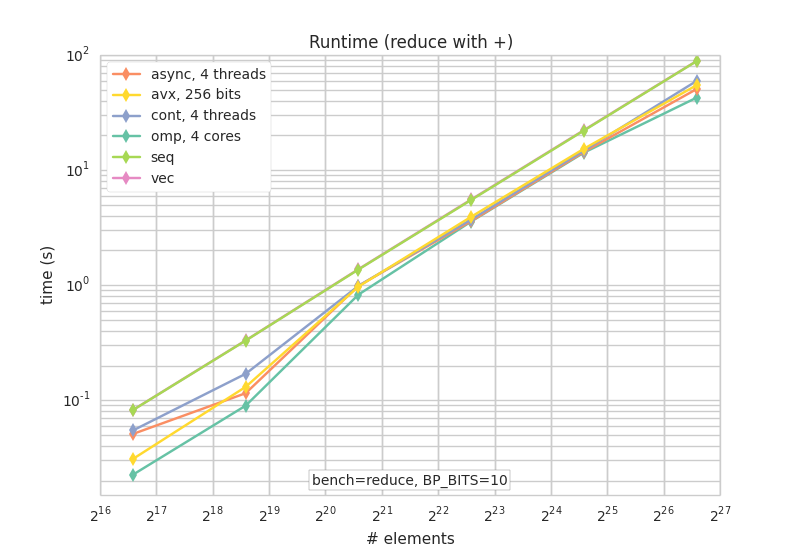
\includegraphics[width=0.5\textwidth]{graphs/cont-reduce_sz-vs-time.png}
\end{figure}
\begin{figure}[!h]
\centering
    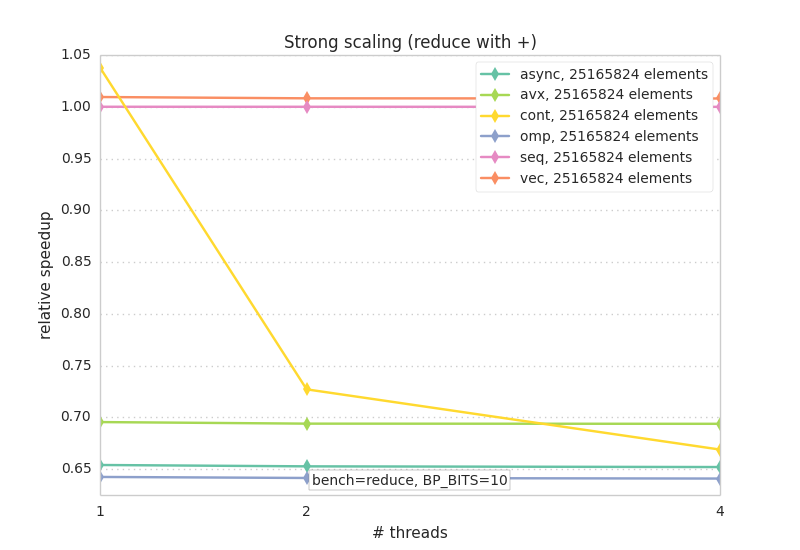
\includegraphics[width=0.5\textwidth]{graphs/cont-reduce-large_procs-vs-speedup.png}
\end{figure}

\subsection{Foreach}
Results show timing for the contentious library performing a foreach operation
on a random vector of doubles. For comparison, the results show the runtime of a
serial implementation as well.

\begin{figure}[!h]
\centering
    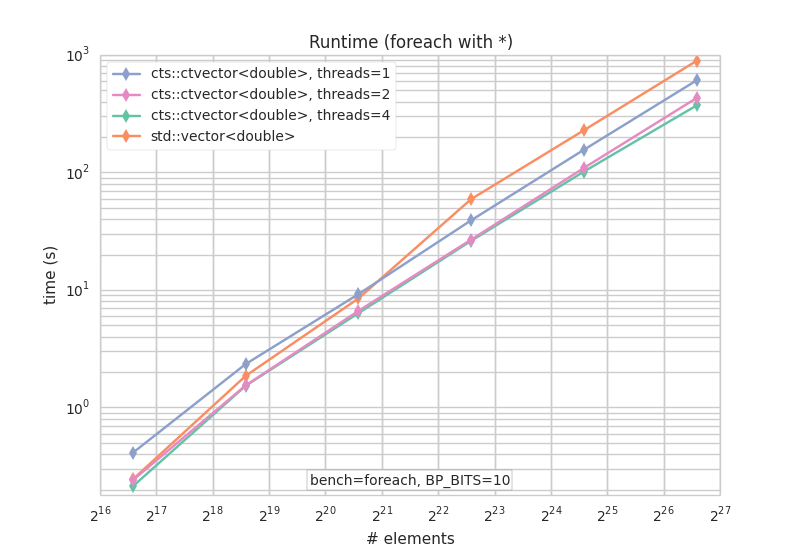
\includegraphics[width=0.5\textwidth]{graphs/cont-foreach_sz-vs-time.png}
\end{figure}
\begin{figure}[!h]
\centering
    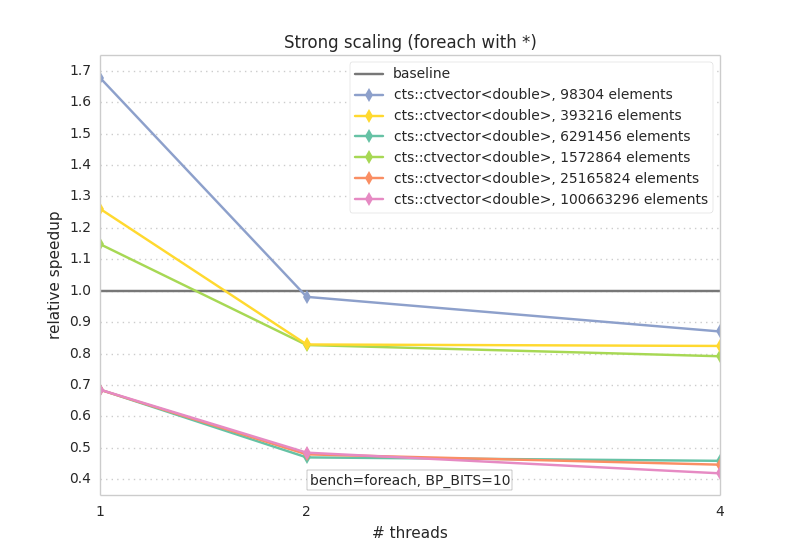
\includegraphics[width=0.5\textwidth]{graphs/cont-foreach_procs-vs-speedup.png}
\end{figure}

\section{Discussion}

The lack of explicit contention management serves as perhaps the most attractive
aspect of postemptive strategies. When using preemptive strategies, the
correctness of the program depends on the ability of the programmer to
explicitly manage concurrent reads and writes of shared data. Historically it
has proven a time-consuming and complex task. Postemptive concurrency control
schemes avoid the need for this and allow for reads and writes to shared data
under common and practical use cases. Their downsides involve potential
decreases in the runtime and space efficiency of the program and the need to
supply extra information about the behavior of the program. But, in practical
settings, it remains to be seen whether postemptive methods such as the one
described competes with optimized preemptive methods.

\subsection{Optimization of Implementation}
There are a number of existing optimizations to CT vectors that are not present
in the current implementation.

\subsubsection{Tail Optimization}
The CT vector can benefit from a tail optimization where the pointer to
the final leaf is stored in the root. This optimization primarily benefits
inserting at the end of the tree, and since the CT vector was primarily
leveraged for mutations as opposed to inserting and removing elements, this
optimization was not prioritized.

\subsubsection{Branching Factor}
The CT vector's nodes stores a constant number of branches or values where that
constant is some power of 2, in order to provide an efficient method for lookup
of values through the tree. When the constant is 32 or greater, the runtime of
traveling to a leaf is at most $\log_{32}(n)$ where $n$ is the size of the
vector. It is unfeasible to store more than 256 billion bytes in memory (this
corresponds to a processor that has access to 256 gigabytes of shared memory),
and it is unrealistic to store objects smaller than one byte.
$\log_{32}(256,000,000,000) \approx 7.58$, which means that the depth of the
bit-partitioned trie of nodes and leaves will never exceed 8. With a branching
factor of 64 and a vector with at most 1 billion values, the depth will never
exceed 5. This growth is so slow that it can, for all intents and purposes, be
treated as a constant, which is why a large branching factor is used. But, the
larger the branching factor, the larger the copy when a CT vector sets a value
in a node it has not yet touched, as it must copy entire nodes. Picking a
contextually good branching factor, or even dynamically determining it or using
heterogeneous branching factors for different parts of the trie, could improve
performance.

\subsubsection{Computation Ordering to Minimize Contention}
When the range of the indexmap is partitioned among splinters, the domain does
not necessarily partition in the same way. Any values in the domain that lie
outside a given splinter's range are candidates for conflicts. These are the
values checked in the resolution process. By having splinters compute these
values first, the chance that conflicts will occur is minimized. This
optimization has not been implemented, and it remains to be seen if the extra
logic necessary to compute the values in a non-consecutive order can be
implemented without the overhead outweighing the benefits.  It is likely that
there are cases, such as multi-dimensional finite difference stencils, where the
sparsity and pattern of values with potential conflicts are straightfoward
enough to easily prioritize.

\subsubsection{Fully lock-free Reattaching and Resolution}
Currently the CT vector implementation uses 2 locks: one to lock the map where
trackers are stored when they are emplaced into the map, and another to lock the
dependent vector's bit-partitioned trie when reattaching of reduce-style
partitions and when resolution happens. The first lock is necessary and does not
affect performance, because the emplacement of values into this map
and lookups in the map accounts for very little actual work compared to the
amount of work splinters would do in actual uses cases for parallelisim. The
second lock has two uses. In the first, really a single processor should perfrom
this reattachment, because each processor holding a lock to perform the final
reduce of $P$ or fewer values incurs substantial overhead compared to a simple
serial reduce. In the second, locking prevents the need to resolve again with
the same dependee-dependent pair after resolution takes place if an output
vector depends on multiple input vectors. The code has not yet been configured
to rerun resolution in the correct sequence to avoid this lock, although as
described it is possible to achieve resolution in a totally
lock-free manner.

The only other synchronization primitive used is a
\texttt{std::atomic<int32\_t>} for assigning ids to CT vectors (and raw
transient vectors, if used).

\subsection{Improvement of Interface}

\subsubsection{The Copying Problem}
CT vectors do not enjoy being copied by value. Currently when you call the copy
constructor on a CT vector, you get a copy of the underlying bit-partitioned
vector with a new id and an otherwise empty set of members. Passing a CT vector
by value to a method and expecting it to behave like a genuine copy of the
original vector does not work. It will not be able to serve as a candidate for
detaching or reattaching splinters as if it were the original vector, and
additionally will not be able to serve as a base for resolution of vectors that
were produced by using the original vector as input. This is, of course, the
correct behavior, but accidentally calling the copy constructor in various
situations may confuse users.

Developing a better interface and writing a semantically correct move
constructor would solve this problem.

\subsubsection{The Intermediate Dependencies Problem}
One major concern involves
writing subroutines that perform multiple stepwise computations (where each step
involves a set of splinter detach and reattach calls) from a local function
scope, where the function returns the final output vector. In order to preserve
the asynchronous properties of the CT vector, the intermediate functions must
be resolved outside the local function scope, or else the resolution will be
premature and force synchronization when the function returns. But, there is no
good way of moving those intermediate CT vectors outside of the local function.
Currently, the destructor of the CT vector waits for all detached splinters to
reattach, as otherwise, segfaults will take place while the splinters do try to
reattach. The destructor does not perform forward resolution or wait for itself
to be resolved; doing so would prevent the desired asynchronous properties.
Resolving onto a vector that has been destroyed (by being \texttt{delete}d if
allocated on the heap, or by going out of scope) is currently undefined behavior
in the same way that using any deleted object is undefined behavior. This is why
the interface requires that the vectors being resolved onto are passed manually
as parameters: it forces users to have undeleted and in scope references eto
them in order to perform resolution on them.

\section{Acknowledgements}
The original idea to use persistent and transient data structures in other
settings came from very useful conversations with Matt Rocklin, who was my
student mentor at the University of chicago before he graduated. My advisor,
Ridgway Scott, and my classmate, Hannah Morgan, both contributed thoughts and
direction, as well as listened patiently to me formulate my ideas out loud.
Another student, Daniel Reid, provided a valuable skepical perspective on
automated synchronization. Finally, without Chris Okazaki's book Purely
Functional Data Structures or Rich Hickey's work on Clojure (and the
corresponding talks), there would be no groundwork for this paper in the first
place.

\bibliographystyle{plain}
\bibliography{references}

\end{document}
